\documentclass[conference]{IEEEtran}
\IEEEoverridecommandlockouts
\usepackage{cite}
\usepackage{amsmath,amssymb}
\usepackage{graphicx}
\usepackage{booktabs}
\usepackage{url}
\usepackage[hidelinks]{hyperref}
\usepackage{tikz}
\usetikzlibrary{positioning,arrows.meta,calc}
\usepackage{tabularx}
\usepackage{float}
\usepackage{placeins}
% Compact, consistent spacing around floats and captions
\setlength{\textfloatsep}{8pt plus 2pt minus 2pt}
\setlength{\floatsep}{6pt plus 2pt minus 2pt}
\setlength{\intextsep}{6pt plus 2pt minus 2pt}
\setlength{\abovecaptionskip}{3pt}
\setlength{\belowcaptionskip}{0pt}
\begin{document}
\title{Uncertainty-Aware Super-Resolution of Satellite Aerosol Data for Air Pollution Mapping}
\author{\IEEEauthorblockN{Ryan Seidel and Rency Ajit Kansagra}
\IEEEauthorblockA{CSE 6367 Computer Vision, Instructor: Dr.\ Diego Patino\\
Department of Computer Science and Engineering, University of Texas at Arlington}}
\maketitle
\begin{abstract}
Air pollution over large areas is often measured using satellites. Satellite images, however, are often too coarse for city-scale features such as an isolated highway. In this project, deep learning super-resolution (SR) is used to sharpen satellite aerosol optical depth (AOD) maps over the Dallas--Fort Worth (DFW) area. Besides the sharp map, the model outputs a per-pixel confidence map, and the sharp AOD is constrained so that averaging it in \(s\times s\) blocks recovers the coarse satellite input. We test against held-out 1\,km MAIAC maps and EPA ground monitors. This midterm report describes the completed data pipeline (six years of daily MAIAC AOD downloaded, clipped, patched, and split by year), the shared residual SR framework with three architectures, and the process by which per-pixel uncertainty is predicted and calibrated. On a preliminary June 2023 split, all three models beat bicubic interpolation (best RMSE 0.0140 vs.\ 0.0147), and their confidence maps are reasonably calibrated on average (90\% coverage 0.83--0.89) but overconfident near clouds.
\end{abstract}
\begin{IEEEkeywords}
super-resolution, remote sensing, aerosol optical depth, PM$_{2.5}$, uncertainty, calibration
\end{IEEEkeywords}
\section{Problem Description}
\subsection{Motivation}
Fine particles in the air, too small for the human eye to see, called PM$_{2.5}$, are one of the biggest environmental health risks. Levels can vary substantially within a few blocks, and busy roads are common hotspots. Although the Environmental Protection Agency (EPA) has ground monitors that measure PM$_{2.5}$ accurately, they are sparse, so most neighborhoods are not directly measured. Satellites address this gap by measuring aerosol optical depth (AOD), which quantifies how much airborne particles block sunlight. AOD is already a primary input for estimating PM$_{2.5}$ across the U.S.~\cite{di2019ensemble}. Even the MAIAC product, one of the sharpest at 1\,km per pixel~\cite{lyapustin2018maiac}, is too coarse to resolve pollution along a single road; many other aerosol products are several kilometers per pixel. Launching higher-resolution satellites is expensive, so we ask whether computer vision can extract more detail from existing data via super-resolution. For the sharp map to be useful, it must remain consistent with the coarse observation and indicate where the model is uncertain.
\begin{figure}[!b]
\centering
\definecolor{c1f}{HTML}{F1EFE8}\definecolor{c1d}{HTML}{8A887F}
\definecolor{c2f}{HTML}{EEEDFE}\definecolor{c2d}{HTML}{7F77DD}
\definecolor{c3f}{HTML}{E1F5EE}\definecolor{c3d}{HTML}{1D9E75}
\definecolor{c4f}{HTML}{FAECE7}\definecolor{c4d}{HTML}{D85A30}
\definecolor{c5f}{HTML}{FAEEDA}\definecolor{c5d}{HTML}{BA7517}
\definecolor{c6f}{HTML}{E6F1FB}\definecolor{c6d}{HTML}{378ADD}
\definecolor{c7f}{HTML}{EAF3DE}\definecolor{c7d}{HTML}{639922}
\resizebox{0.95\columnwidth}{!}{%
\begin{tikzpicture}[
    node distance=0.45cm,
    st/.style={draw=#1d, fill=#1f, rounded corners=3pt, align=center, minimum height=1.0cm, text width=3.6cm, line width=0.5pt},
    sm/.style={draw=#1d, fill=#1f, rounded corners=3pt, align=center, minimum height=1.0cm, text width=2.8cm, line width=0.5pt},
    ln/.style={draw=gray!70, line width=0.5pt}]
  \newcommand{\bx}[2]{{\small #1}\\[-1pt]{\scriptsize #2}}
  \node[st=c1] (a) {\bx{Low-res satellite images}{input data}};
  \node[st=c2, below=of a] (b) {\bx{Prepare data}{cut into small patches}};
  \node[st=c3, below=of b] (c) {\bx{AI model (SR)}{sharp map + confidence}};
  \node[sm=c4, below left=0.8cm and -1.3cm of c] (d) {\bx{Sharp image}{1\,km AOD}};
  \node[sm=c5, below right=0.8cm and -1.3cm of c] (e) {\bx{Confidence map}{how sure it is}};
  \node[st=c6, anchor=north] (f) at ($(c.south |- d.south)+(0,-0.75)$) {\bx{Compare to real image}{accuracy + re-average check}};
  \node[st=c7, below=of f] (g) {\bx{Improve the model}{adjust and retrain}};
  \draw[ln] (a) -- (b);
  \draw[ln] (b) -- (c);
  \draw[ln] (c.south) -- ++(0,-0.4) coordinate (s1);
  \draw[ln] (d.north |- s1) -- (e.north |- s1);
  \draw[ln] (d.north |- s1) -- (d.north);
  \draw[ln] (e.north |- s1) -- (e.north);
  \draw[ln] (d.south) -- ++(0,-0.35) coordinate (s2) -- (e.south |- s2) -- (e.south);
  \draw[ln] (f.north |- s2) -- (f.north);
  \draw[ln] (f) -- (g);
  \draw[ln, dashed, gray!60] (c.east) -- ($(e.east |- c.east)+(0.4,0)$) coordinate (r1) -- (r1 |- g.east) node[pos=0.55, right, font=\scriptsize, text=gray!90!black]{$\circlearrowright$ retrain loop} -- (g.east);
\end{tikzpicture}}
\caption{Project pipeline. The sharp map is also averaged back to the coarse input.}
\label{fig:pipeline}
\end{figure}
\subsection{Super-Resolution as a Computer Vision Problem}
Super-resolution (SR) recovers a high-resolution (HR) image from a low-resolution (LR) observation. The problem is underdetermined: many HR images can map to the same LR input~\cite{wang2021survey}. Recent SR architectures have shifted from convolutional neural networks (CNNs) toward transformer-based designs such as HAT~\cite{chen2023hat}. SR has been applied to satellite imagery, mostly from Sentinel-2~\cite{lanaras2018dsen2,nguyenvi2025channel,massarelli2026interp}, and to multi-frame sequences of the same area~\cite{deudon2020highresnet}; an overview appears in~\cite{digitalsense_blog}. Two limitations are relevant here. First, SR models can ``hallucinate'' details that look plausible but are not present, so consistency with the input is helpful~\cite{aybar2026sen2sr,massarelli2026interp}. Second, a better PSNR or SSIM does not always imply better downstream utility~\cite{shermeyer2019effects}. Most existing satellite SR work sharpens photographic imagery rather than measurement maps such as AOD. For AOD we enforce the consistency constraint explicitly: averaging the 1\,km output in \(s\times s\) blocks must recover the coarse input.
\subsection{Challenge}
Sharpening an AOD map is harder than sharpening a natural photograph. The mapping is one-to-many, AOD fields lack sharp edges (so gradient or Laplacian losses may not help), and clouds produce missing pixels in both inputs and targets. Training data are imbalanced: high-pollution days (e.g., wildfire smoke) are rare yet most important for health. Finally, there is no true high-resolution answer key for genuinely coarse satellite observations.
\subsection{Problem Statement}
Given a low-resolution AOD map \(\mathbf{x}\in\mathbb{R}^{H\times W}\) at \(s\times\)1\,km resolution, we train a network
\begin{equation}
f_\theta:\ \mathbf{x}\ \mapsto\ \big(\hat{\mathbf{y}},\ \hat{\boldsymbol{\sigma}}^2\big),\qquad \hat{\mathbf{y}},\hat{\boldsymbol{\sigma}}^2\in\mathbb{R}^{sH\times sW},
\end{equation}
where \(\hat{\mathbf{y}}\) is the sharpened 1\,km map and \(\hat{\boldsymbol{\sigma}}^2\) is the per-pixel variance. We also enforce \(\mathrm{AvgPool}_{s\times s}(\hat{\mathbf{y}}) \approx \mathbf{x}\). Because the maps may inform public-health decisions, uncertainty estimates must be well calibrated: when the model claims 80\% confidence, the true value should fall inside the predicted interval roughly 80\% of the time. We model aleatoric uncertainty via a predicted per-pixel variance~\cite{kendall2017uncertainties}, following recent SR uncertainty papers~\cite{he2025buff,zhang2025upsr,csillag2024trust} that have so far been evaluated only on natural images. Epistemic uncertainty (e.g., an ensemble of the three backbones) is left as an extension. Our research questions are:
\begin{itemize}
\item \textbf{RQ1 (Accuracy):} Can a deep SR model recover a sharper 1\,km AOD map from a 4\,km input more accurately than bicubic interpolation? Metrics: RMSE, PSNR, SSIM, and a detail ratio, evaluated on held-out 1\,km MAIAC maps.
\item \textbf{RQ2 (Consistency):} Does forcing the sharpened map to average back to the coarse input reduce hallucinated detail without simply re-blurring the map? We compare the same model with the constraint off versus on, reporting \(|\mathrm{AvgPool}(\hat{\mathbf{y}})-\mathbf{x}|\).
\item \textbf{RQ3 (Calibration):} Is the per-pixel uncertainty well calibrated? We report empirical coverage \(C_p\) at several nominal levels and the calibration error.
\item \textbf{RQ4 (Downstream utility):} Does the sharpened 1\,km AOD correlate more strongly with EPA PM$_{2.5}$ monitors than the original coarse 4\,km AOD? We report \(R^2\).
\end{itemize}
We also provide side-by-side visual examples.
\subsection{Scope}
We use public MAIAC AOD, including elevated-AOD smoke days. We sharpen AOD rather than train a surface PM$_{2.5}$ model and do not solve atmospheric transport PDEs; the only physics-based regularizer is the average-back-to-input constraint. RQ4 only checks whether sharper AOD aligns better with monitors~\cite{di2019ensemble}. The required scale factor is \(s{=}4\) (4\,km \(\to\) 1\,km). A road-density auxiliary input, a smoke-day subset, or \(s{=}10\) are stretch goals once the core experiments finish.
\section{Data Description}
\subsection{Satellite Data: MAIAC AOD}
We use NASA's MCD19A2 Collection~6.1 product~\cite{mcd19a2}, which supplies daily 1\,km AOD from Terra (morning) and Aqua (afternoon)~\cite{lyapustin2018maiac}. Files are free HDF granules from NASA Earthdata. DFW lies in tile \texttt{h09v05}. We retain the 550\,nm AOD and quality flags, scale integer values by 0.001, and mask pixels flagged as cloud, snow, or bright surface. Full daily granules were downloaded year by year, clipped to the DFW box, scaled, QA-masked, and written as compact daily arrays. (A Google Earth Engine prototype was also tested.)
\begin{table}[H]
\caption{Summary of Data Sources}
\label{tab:data}
\centering
\footnotesize
\setlength{\tabcolsep}{3pt}
\renewcommand{\arraystretch}{1.0}
\begin{tabularx}{\columnwidth}{@{}l l l >{\raggedright\arraybackslash}X@{}}
\toprule
\textbf{Dataset} & \textbf{Quantity} & \textbf{Resolution} & \textbf{Role} \\
\midrule
MAIAC MCD19A2 & AOD (550\,nm) & 1\,km, daily & HR target \\
Degraded MAIAC & AOD (550\,nm) & \(s\)\,km (\(s{=}4\)) & LR input \\
EPA AQS & Surface PM$_{2.5}$ & Point, hourly/daily & Validation \\
\bottomrule
\end{tabularx}
\end{table}
\subsection{Ground Data: EPA PM$_{2.5}$ Monitors}
For RQ4 we use quality-checked PM$_{2.5}$ readings (parameter code 88101) from the EPA Air Quality System (AQS) API~\cite{epa_aqs}. AQS is preferred over AirNow~\cite{epa_airnow} because the latter is preliminary. Monitors are used only for evaluation, never for training. Pre-built annual AQS files (no login required) were downloaded and filtered to the DFW box. Because Terra and Aqua overpass DFW near 10:30 and 13:30 local time, we average each monitor's hourly values from 10:00--14:00, requiring at least three of the five hours. Multi-instrument sites are averaged so each site contributes once per day.
\subsection{Study Area and Time Period}
The domain is approximately 32.3--33.5$^\circ$N, 97.8--96.3$^\circ$W (2018--2023). At 1\,km the region is only about \(140\times130\) pixels, yielding a modest number of \(64\times64\) patches even with roughly 4{,}000 overpasses. Patches were therefore extracted from the clipped region across all six years.
\subsection{Downloading and Preparing the Data}
One year at a time was retrieved from NASA Earthdata (\(\approx\)365 granules per year), clipped, scaled by 0.001, QA-masked, and stored as compact daily arrays. We then extracted \(64\times64\) patches on a 32-pixel stride, retaining only patches with at least 60\% valid pixels. Each patch stores a \(16\times16\) low-resolution input (masked \(4\times4\) box average of the high-resolution field), a \(64\times64\) high-resolution target, and a binary validity mask. Missing pixels are stored as NaN together with the mask. Representative examples appear in Fig.~\ref{fig:dfw} and Fig.~\ref{fig:patch}.
\begin{figure}[htbp]
\centering
\includegraphics[width=0.50\columnwidth]{dfw_sample.png}
\caption{Example daily MAIAC AOD map (550\,nm, 1\,km) over the DFW box after clipping, scaling, and QA masking. White areas have no retrieval, mostly under clouds.}
\label{fig:dfw}
\end{figure}
\begin{figure}[htbp]
\centering
\includegraphics[width=0.85\columnwidth]{patch_example.png}
\caption{One prepared training patch: the \(64\times64\) HR target, the \(16\times16\) LR input (masked \(4\times4\) box average), and the validity mask (black = missing).}
\label{fig:patch}
\end{figure}
The year-based split and train-only normalization statistics are complete and stored in the repository (\texttt{data/split\_data/}): 2018--2021 for training, 2022 for validation (checkpoint selection, hyper-parameters, \(\hat\sigma\) rescaling), and 2023 for testing. Mean and standard deviation were computed on the training years only. Scripts for clipping, patch extraction, and the year split reside in \texttt{src/Data extraction/}. A few missing days per year do not affect results.
\section{Methods}
\subsection{A Shared Residual SR Framework}
To enable a fair comparison, every architecture sits inside the same residual wrapper. The input has two channels: the standardized LR AOD and its validity mask. The network body \(g_\theta\) predicts only the residual detail, which is added to a bicubic upsampling of the input:
\begin{equation}
\hat{\mathbf{y}} = \mathrm{Bicubic}_s(\mathbf{x}) + \mathbf{d},\qquad (\mathbf{d},\ \boldsymbol{\ell}) = g_\theta(\mathbf{x},\mathbf{m}),
\end{equation}
where \(\mathbf{m}\) is the validity mask and \(\mathbf{d}\) is the fine-scale residual. The network also emits a log-variance map \(\boldsymbol{\ell}=\log\hat{\boldsymbol{\sigma}}^2\). Predicting the logarithm guarantees positivity; clamping \(\boldsymbol{\ell}\) to \([-10,10]\) stabilizes training. Only the body \(g_\theta\) changes across the three models.
\subsection{Three Architectures}
We evaluate one representative from each major SR family. All models are modest (0.9--1.9M parameters).
\begin{itemize}
\item \textbf{EDSR}~\cite{lim2017edsr}: residual blocks operating at LR resolution followed by PixelShuffle upsampling. Works at \(16\times16\) with deep local filters (1.52M weights).
\item \textbf{U-Net}~\cite{ronneberger2015unet}: bicubic upsampling first, then an encoder-decoder with skip connections. Works at \(64\times64\), shrinking to \(8\times8\) (1.93M weights).
\item \textbf{SwinIR-light}~\cite{liang2021swinir}: shifted-window self-attention. Works at \(16\times16\) (0.92M weights).
\end{itemize}
\subsection{RQ1: Does Super-Resolution Improve Accuracy?}
We take a real 1\,km MAIAC map, deliberately average it into a 4\,km image, and ask the model to recover the higher-resolution image. We then compare that output to the original 1\,km map using RMSE, PSNR, SSIM, and a detail ratio. The baseline is bicubic interpolation.
\begin{figure}[!t]
\centering
\resizebox{\columnwidth}{!}{%
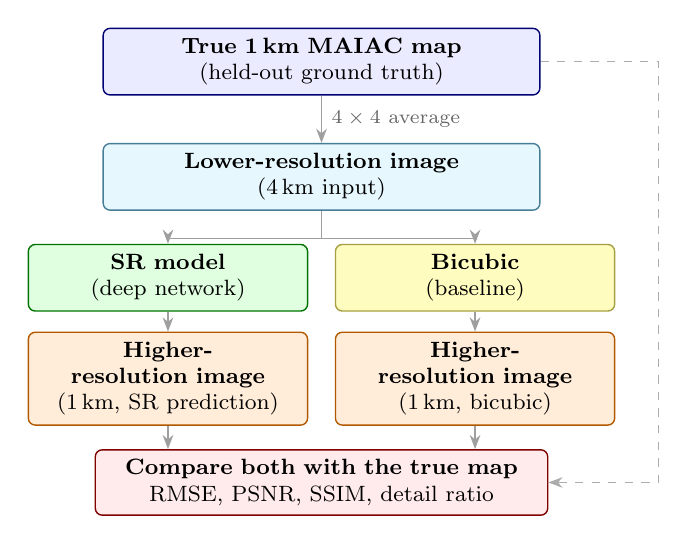
\begin{tikzpicture}[
  font=\footnotesize,
  box/.style={rounded corners=2.5pt, align=center, inner sep=3.5pt, line width=0.5pt, minimum height=0.72cm},
  arr/.style={-{Stealth[length=1.8mm]}, line width=0.55pt, draw=gray!75}
]
\node[box, text width=5.3cm, fill=blue!8, draw=blue!45!black] (truth) {\textbf{True 1\,km MAIAC map}\\(held-out ground truth)};
\node[box, text width=5.3cm, fill=cyan!10, draw=cyan!55!black, below=0.6cm of truth] (lr) {\textbf{Lower-resolution image}\\(4\,km input)};
\node[box, text width=3.3cm, fill=green!12, draw=green!45!black] (sr) at ($(lr.south)+(-1.95,-0.85)$) {\textbf{SR model}\\(deep network)};
\node[box, text width=3.3cm, fill=yellow!25, draw=yellow!60!black] (bic) at ($(lr.south)+(1.95,-0.85)$) {\textbf{Bicubic}\\(baseline)};
\node[box, text width=3.3cm, fill=orange!15, draw=orange!70!black] (hrsr) at ($(sr.south)+(0,-0.85)$) {\textbf{Higher-resolution image}\\(1\,km, SR prediction)};
\node[box, text width=3.3cm, fill=orange!15, draw=orange!70!black] (hrbic) at ($(bic.south)+(0,-0.85)$) {\textbf{Higher-resolution image}\\(1\,km, bicubic)};
\node[box, text width=5.5cm, fill=red!8, draw=red!50!black] (cmp) at ($(lr.south)+(0,-3.45)$) {\textbf{Compare both with the true map}\\RMSE, PSNR, SSIM, detail ratio};
\draw[arr] (truth) -- node[right, font=\scriptsize, text=gray!80!black]{$4\times4$ average} (lr);
\draw[arr] (lr.south) -- ++(0,-0.35) -| (sr.north);
\draw[arr] (lr.south) -- ++(0,-0.35) -| (bic.north);
\draw[arr] (sr) -- (hrsr);
\draw[arr] (bic) -- (hrbic);
\draw[arr] (hrsr.south) -- (cmp.north -| hrsr.south);
\draw[arr] (hrbic.south) -- (cmp.north -| hrbic.south);
\coordinate (lane) at ($(truth.east)+(1.5,0)$);
\draw[arr, dashed, draw=gray!65] (truth.east) -- (lane) -- (lane |- cmp.east) -- (cmp.east);
\end{tikzpicture}}
\caption{RQ1: the true 1\,km map is degraded to a 4\,km image; the SR model and bicubic baseline each produce a 1\,km map that is scored against the original true map.}
\label{fig:rq1}
\end{figure}
\subsection{RQ2: Does the Average-Back Constraint Help?}
We run the same model twice: once with the average-back constraint off and once with it on. The constraint forces the higher-resolution image to average back to the original lower-resolution input. We compare accuracy and the amount of invented detail. In training the constraint is an extra penalty \(\mathcal{L}=\mathcal{L}_{\mathrm{NLL}}+\lambda\,\mathcal{L}_{\mathrm{avg}}\).
\begin{figure}[!t]
\centering
\resizebox{\columnwidth}{!}{%
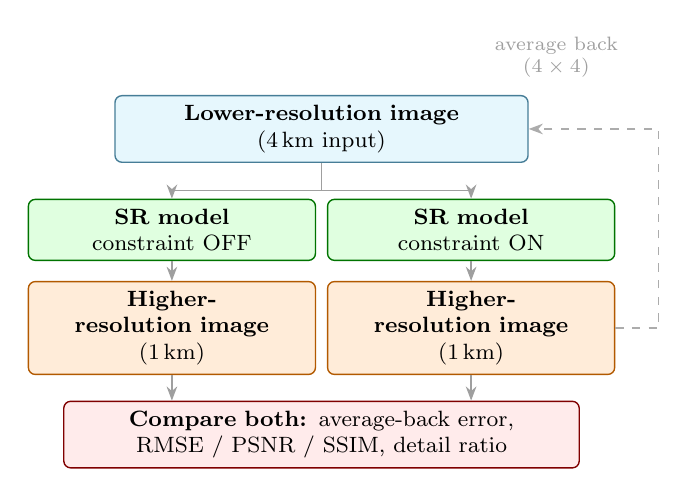
\begin{tikzpicture}[
  font=\footnotesize,
  box/.style={rounded corners=2.5pt, align=center, inner sep=3.5pt, line width=0.5pt, minimum height=0.72cm},
  arr/.style={-{Stealth[length=1.8mm]}, line width=0.55pt, draw=gray!75}
]
\node[box, text width=5.0cm, fill=cyan!10, draw=cyan!55!black] (lr) {\textbf{Lower-resolution image}\\(4\,km input)};
\node[box, text width=3.4cm, fill=green!12, draw=green!45!black] (off) at ($(lr.south)+(-1.9,-0.85)$) {\textbf{SR model}\\constraint OFF};
\node[box, text width=3.4cm, fill=green!12, draw=green!45!black] (on) at ($(lr.south)+(1.9,-0.85)$) {\textbf{SR model}\\constraint ON};
\node[box, text width=3.4cm, fill=orange!15, draw=orange!70!black] (hroff) at ($(off.south)+(0,-0.85)$) {\textbf{Higher-resolution image}\\(1\,km)};
\node[box, text width=3.4cm, fill=orange!15, draw=orange!70!black] (hron) at ($(on.south)+(0,-0.85)$) {\textbf{Higher-resolution image}\\(1\,km)};
\node[box, text width=6.3cm, fill=red!8, draw=red!50!black] (cmp) at ($(lr.south)+(0,-3.45)$) {\textbf{Compare both:} average-back error,\\RMSE / PSNR / SSIM, detail ratio};
\draw[arr] (lr.south) -- ++(0,-0.35) -| (off.north);
\draw[arr] (lr.south) -- ++(0,-0.35) -| (on.north);
\draw[arr] (off) -- (hroff);
\draw[arr] (on) -- (hron);
\draw[arr] (hroff.south) -- (cmp.north -| hroff.south);
\draw[arr] (hron.south) -- (cmp.north -| hron.south);
\coordinate (lane2) at ($(hron.east)+(0.55,0)$);
\draw[arr, dashed, draw=gray!65] (hron.east) -- (lane2) -- (lane2 |- lr.east) -- (lr.east);
\node[above, font=\scriptsize, text=gray!75, align=center] at ($(lr.north east)+(0.35,0.1)$) {average back\\($4\times4$)};
\end{tikzpicture}}
\caption{RQ2: the same 4\,km input is sharpened with the average-back constraint off and on. The dashed loop averages the 1\,km output and penalizes mismatch with the input; both outputs are compared on consistency, accuracy, and detail.}
\label{fig:rq2}
\end{figure}
\subsection{How Uncertainty Is Obtained (RQ3)}
Uncertainty is obtained by heteroscedastic regression. The network jointly predicts the mean map \(\hat{\mathbf{y}}\) and the log-variance map \(\boldsymbol{\ell}=\log\hat{\boldsymbol{\sigma}}^2\). Training minimizes the Gaussian negative log-likelihood~\cite{kendall2017uncertainties} averaged over valid pixels \(\mathcal{M}\):
\begin{equation}
\mathcal{L}_{\mathrm{NLL}} = \frac{1}{|\mathcal{M}|}\sum_{i\in\mathcal{M}} \tfrac{1}{2}\Big(e^{-\ell_i}\,(y_i-\hat y_i)^2 + \ell_i\Big).
\end{equation}
\begin{figure}[!t]
\centering
\resizebox{\columnwidth}{!}{%
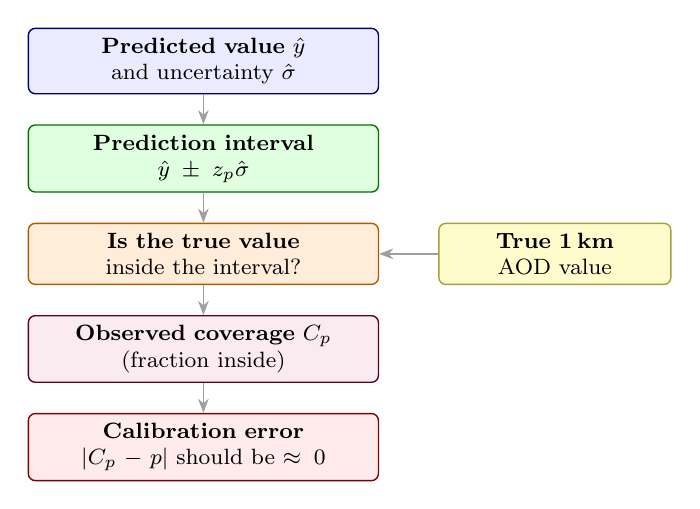
\begin{tikzpicture}[
  font=\footnotesize,
  box/.style={rounded corners=2.5pt, align=center, inner sep=3.5pt, line width=0.5pt, minimum height=0.72cm},
  arr/.style={-{Stealth[length=1.8mm]}, line width=0.55pt, draw=gray!75}
]
\node[box, text width=4.2cm, fill=blue!8, draw=blue!45!black] (pred) {\textbf{Predicted value \(\hat y\)}\\and uncertainty \(\hat\sigma\)};
\node[box, text width=4.2cm, fill=green!12, draw=green!45!black, below=0.38cm of pred] (int) {\textbf{Prediction interval}\\\(\hat y \pm z_p\hat\sigma\)};
\node[box, text width=4.2cm, fill=orange!15, draw=orange!70!black, below=0.38cm of int] (chk) {\textbf{Is the true value}\\inside the interval?};
\node[box, text width=2.7cm, fill=yellow!20, draw=yellow!60!black, right=0.75cm of chk] (truth) {\textbf{True 1\,km}\\AOD value};
\node[box, text width=4.2cm, fill=purple!8, draw=purple!50!black, below=0.38cm of chk] (cov) {\textbf{Observed coverage \(C_p\)}\\(fraction inside)};
\node[box, text width=4.2cm, fill=red!8, draw=red!50!black, below=0.38cm of cov] (cal) {\textbf{Calibration error}\\\(|C_p - p|\) should be \(\approx 0\)};
\draw[arr] (pred) -- (int);
\draw[arr] (int) -- (chk);
\draw[arr] (truth) -- (chk);
\draw[arr] (chk) -- (cov);
\draw[arr] (cov) -- (cal);
\end{tikzpicture}}
\caption{RQ3: predicted uncertainty is turned into a prediction interval, the true AOD is checked against it, and observed coverage \(C_p\) is compared with the claimed level \(p\).}
\label{fig:rq3flow}
\end{figure}
At test time we recover \(\hat{\sigma}=\exp(\ell/2)\) and form prediction intervals. Coverage \(C_p\) and calibration error are reported. A single scalar recalibration factor can be fitted on the 2022 validation year and applied to \(\hat\sigma\).
\subsection{Evaluation Metrics}
All scores ignore missing (cloud) pixels; Table~\ref{tab:eval} summarizes the plan.
\begin{table}[htbp]
\caption{Evaluation plan (all on the 2023 test year)}
\label{tab:eval}
\centering
\footnotesize
\setlength{\tabcolsep}{2pt}
\begin{tabularx}{\columnwidth}{@{}l l l >{\raggedright\arraybackslash}X@{}}
\toprule
\textbf{RQ} & \textbf{What we measure} & \textbf{Compared against} & \textbf{Success looks like} \\
\midrule
RQ1 & RMSE, PSNR, SSIM, detail & Bicubic & Lower error than bicubic \\
RQ2 & Avg-back error + detail & Constraint off & Less invented detail, little accuracy drop \\
RQ3 & Coverage \(C_p\), calib.\ error & Nominal \(p\) & \(C_p\approx p\) \\
RQ4 & All-days and within-day \(R^2\) & Coarse 4\,km AOD & Higher \(R^2\) with EPA PM$_{2.5}$ \\
\bottomrule
\end{tabularx}
\end{table}
\textbf{RQ1:} Besides RMSE, PSNR, and SSIM~\cite{wang2004ssim}, we report a \emph{detail ratio} (how much fine-scale variation the model recovers versus invents), computed as the fine-scale variation of the prediction divided by that of the true map, where fine-scale means what \(4\times4\) averaging removes. A value near 1.0 is ideal; below 1 means too smooth and above 1 means invented detail.
\textbf{RQ2:} The average-back error is the root-mean-square gap between the block-averaged output and the lower-resolution input, reported with and without the constraint.
\textbf{RQ3:} The coverage \(C_p\) is the fraction of valid pixels whose true value lies inside the interval at level \(p\). The calibration error is the average of \(|C_p-p|\) over \(p\in\{0.5,0.8,0.9,0.95\}\), and we also report the mean interval width, since very wide intervals can reach the right coverage without being useful.
\textbf{RQ4:} We compute \(R^2\) between AOD and PM$_{2.5}$ in two ways. The all-days \(R^2\) shows whether AOD tracks overall haze level. The within-day \(R^2\) (after subtracting each day's DFW-wide average) shows whether extra resolution helps explain which locations are cleaner or dirtier on the same day.
\section{Preliminary Results}
All numbers use a temporary June 2023 date split (112 train / 32 validation patches). Models are trained with Adam (learning rate \(2\times10^{-4}\), batch size 32). The average-back constraint is switched off for these runs. Final numbers will use the 2018--2021/2022/2023 year split.
\subsection{Sanity Check and RQ1}
Each model was first trained to memorize a single high-variation patch (Table~\ref{tab:onepatch}). All three succeeded. On the 32 held-out validation patches (Table~\ref{tab:rq1}) every model beats bicubic; the best reaches RMSE 0.0140 versus 0.0147. The detail ratio rises from 0.32 (bicubic) to \(\approx0.5\), so the models add real texture rather than pure hallucination, although the true maps still contain roughly twice as much fine detail.
\begin{table}[htbp]
\caption{One-patch memorization test}
\label{tab:onepatch}
\centering\footnotesize
\begin{tabular}{lcccc}
\toprule
 & Bicubic & EDSR & U-Net & SwinIR-light \\
\midrule
RMSE & 0.0235 & 0.00017 & 0.00033 & 0.00040 \\
Detail ratio & 0.24 & 1.00 & 1.00 & 1.00 \\
\bottomrule
\end{tabular}
\end{table}
\begin{table}[htbp]
\caption{RQ1 on 32 validation patches}
\label{tab:rq1}
\centering\footnotesize
\begin{tabular}{lcccc}
\toprule
Method & RMSE$\downarrow$ & PSNR$\uparrow$ & SSIM$\uparrow$ & Detail \\
\midrule
Bicubic & 0.0147 & 36.68 & 0.891 & 0.32 \\
EDSR & 0.0142 & 36.92 & 0.902 & 0.53 \\
U-Net & 0.0142 & 36.93 & 0.900 & 0.40 \\
SwinIR-light & \textbf{0.0140} & \textbf{37.10} & \textbf{0.905} & 0.54 \\
\bottomrule
\end{tabular}
\end{table}
\subsection{RQ3: Calibration of the Confidence Map}
On average the maps are reasonably calibrated (90\% coverage 0.83--0.89, calibration error 0.02--0.04). Coverage drops near cloud edges and is worst on the most confident pixels (Table~\ref{tab:rq3}). Fig.~\ref{fig:rq3} shows the calibration curves and the bootstrap ranges on the 32 validation patches. Coverage is unstable across epochs, the most confident third of pixels is the least well covered, and the three consecutive validation days do not include smoke events.
\begin{figure}[htbp]
\centering
\includegraphics[width=0.85\columnwidth]{rq3_fig.png}
\caption{RQ3 check on the June 2023 validation patches. Left: calibration curves (below the dashed line = overconfident). Right: 90\% coverage with bootstrap range over the 32 patches (the range understates true uncertainty because the patches come from only three days).}
\label{fig:rq3}
\end{figure}
\begin{table}[htbp]
\caption{RQ3: 90\% coverage (target 0.90)}
\label{tab:rq3}
\centering\footnotesize
\begin{tabular}{lcccc}
\toprule
Model & All & Cal.\ err. & Cloud edge & Most sure \\
\midrule
EDSR & 0.889 & 0.019 & 0.84 & 0.88 \\
U-Net & 0.867 & 0.017 & 0.82 & 0.84 \\
SwinIR-light & 0.833 & 0.041 & 0.81 & 0.77 \\
\bottomrule
\end{tabular}
\end{table}
\subsection{RQ4: Relation to Ground PM$_{2.5}$}
Raw AOD correlates with midday EPA PM$_{2.5}$ at \(R^2\approx0.3\), but 1\,km and 4\,km versions perform almost identically and within-day \(R^2\) is near zero (Fig.~\ref{fig:rq4}). With only 21 unseen monitor-days the current data cannot yet answer RQ4. At the monitors the 1\,km and 4\,km values differ by only 0.016 on average, while day-to-day AOD variation is larger (\(\approx0.068\)).
\begin{figure}[!ht]
\centering
\includegraphics[width=0.85\columnwidth]{rq4_fig.png}
\caption{RQ4 first look: AOD vs.\ ground PM$_{2.5}$, DFW June 2023. Top row: all 88 monitor-days. Bottom row: within-day anomalies (81 monitor-days on 14 days). 1\,km resolution does not improve the correlation relative to the native 4\,km average.}
\label{fig:rq4}
\end{figure}
\FloatBarrier
\section{Implementation Status and Contributions}
The data extraction, clipping, patch generation, and leakage-free year split (with train-only statistics) are complete and available in the repository under \texttt{data/split\_data/} and \texttt{src/Data extraction/} (Rency). Figs.~\ref{fig:dfw} and~\ref{fig:patch} are produced directly from these files, so the pipeline runs end to end from raw granules to model-ready patches. The shared residual wrapper, three model backbones, NLL and average-back losses, and evaluation code are implemented (Ryan). Training and the full RQ1--RQ4 experiments can now begin on the ready split data. Prior to large-scale training, each model will be double-checked by memorizing a single patch.
\section{Risks and Open Questions}
Time is the main risk. If training runs long we will still keep 2023 strictly held out. A second risk is that the gain over bicubic may be modest because AOD maps are smooth; that remains a valid answer to RQ1 and RQ4. 
A major risk specific to RQ3 is that the predicted uncertainty may be poorly calibrated. Heteroscedastic models can under- or over-estimate variance, especially on high-AOD or cloudy days, so the coverage \(C_p\) may deviate substantially from the nominal level \(p\). If this occurs, the confidence map would be less useful for decision-making even if the mean prediction is accurate. We mitigate this by evaluating full calibration curves on the held-out year, applying a simple scalar recalibration on the validation year if needed, and reporting coverage separately for high-AOD and near-cloud pixels.
Open questions include whether RQ1 should use plain masked MSE or the joint uncertainty loss, and whether all three architectures are needed if they perform similarly. A model trained on our own degraded inputs may behave differently on real coarse satellite data~\cite{aybar2026sen2sr}, which we will note as a limitation.

% ======================================================================
% FINAL RESULTS (added after the midterm report; everything above is unchanged)
% Figures live in final_paper/ ; new references are in final_paper/new_refs.bib
% ======================================================================
\section{Final Results on the Year Split}
All numbers in this section use the year split described in Section~II: training on 2018--2021 (4{,}543 patches), checkpoint and calibration choices on 2022 (1{,}142 patches), and a single evaluation on 2023 (976 patches). The 2023 year is never used for training or for choosing anything. Models are trained with Adam (learning rate \(2\times10^{-4}\), batch size 32) and the NLL loss of Eq.~(3). Table~\ref{tab:summary} summarizes the answers; the subsections below give the details.

\begin{table}[htbp]
\caption{Summary of findings on the 2023 test year}
\label{tab:summary}
\centering\footnotesize
\setlength{\tabcolsep}{3pt}
\renewcommand{\arraystretch}{1.1}
\begin{tabularx}{\columnwidth}{@{}l >{\raggedright\arraybackslash}X >{\raggedright\arraybackslash}X@{}}
\toprule
\textbf{RQ} & \textbf{Answer} & \textbf{Key numbers} \\
\midrule
RQ1 & Yes: every model beats bicubic; SwinIR-light is best on all five seeds. & RMSE 0.0107 vs.\ 0.0126 (\(-15\%\)); PSNR +1.4\,dB \\
RQ2 & Yes: exact consistency with no loss of accuracy or detail. & Avg-back error \(\le\)2e-3 \(\to\) 8.7e-9; detail 0.64--0.74 \(\to\) 0.71--0.75 \\
RQ3(a) & Yes: \(\hat\sigma\) points at the pixels the model gets wrong, but raw \(\hat\sigma\) can be overconfident. & Error rises 5--7\(\times\) across \(\hat\sigma\) groups; 90\% coverage 0.79--0.91 \\
RQ3(b) & Yes: one scale factor fitted on 2022 gives a range that holds on 2023 for every model. & 6.4--7.7\% misses (target \(\le\)10\%); cloud-edge misses 8--13\% vs.\ 17--20\% for a constant range \\
Fix & Pick the epoch by NLL (free); a 5-model ensemble is best overall. & SwinIR coverage 0.79 \(\to\) 0.87; ensemble RMSE 0.0104, coverage 0.91 \\
% RQ4 & (Rency) & \\
\bottomrule
\end{tabularx}
\end{table}

\textbf{Role of the bicubic baseline (Fig.~\ref{fig:rq1}).} Bicubic interpolation is a fixed formula with no training. It receives only the same 4\,km input as the SR model and never sees the true 1\,km map. Both outputs are scored against the same held-out map, so the gap between them measures what learning adds. The true map is never an input to either method: it is used only to build the 4\,km input, as the training target (2018--2021), and for scoring (2023). Because our networks predict a residual on top of bicubic (Eq.~(2)), beating bicubic directly measures the value of the learned detail \(\mathbf{d}\).

\subsection{RQ1 and RQ2: Accuracy and the Average-Back Constraint}
In the final runs the average-back constraint is applied as a hard correction after the network, \(\hat{\mathbf{y}} \leftarrow \hat{\mathbf{y}} + \mathrm{Up}_s\big(\mathbf{m}\odot(\mathbf{x}-\mathrm{AvgPool}_s(\hat{\mathbf{y}}))\big)\), where \(\mathrm{Up}_s\) copies each coarse value to its \(s\times s\) block. Table~\ref{tab:final} reports each model trained once for 200 epochs with the epoch picked by 2022 RMSE.

\begin{table}[htbp]
\caption{RQ1 and RQ2 on the 2023 test year (one run per model)}
\label{tab:final}
\centering\footnotesize
\setlength{\tabcolsep}{3pt}
\resizebox{\columnwidth}{!}{%
\begin{tabular}{lccccc}
\toprule
Method & RMSE$\downarrow$ & PSNR$\uparrow$ & SSIM$\uparrow$ & Detail & Avg-back err.$\downarrow$ \\
\midrule
Bicubic & 0.0126 & 37.97 & 0.927 & 0.49 & -- \\
EDSR & 0.0116 & 38.71 & 0.940 & 0.64 & 1.5e-3 \\
EDSR + constraint & 0.0109 & 39.24 & 0.948 & 0.71 & 8.7e-9 \\
U-Net & 0.0110 & 39.14 & 0.948 & 0.72 & 1.7e-3 \\
U-Net + constraint & 0.0110 & 39.21 & 0.949 & 0.73 & 8.7e-9 \\
SwinIR-light & \textbf{0.0107} & \textbf{39.42} & \textbf{0.951} & 0.74 & 6.4e-4 \\
SwinIR-light + constraint & \textbf{0.0107} & 39.40 & \textbf{0.951} & 0.75 & 8.7e-9 \\
\bottomrule
\end{tabular}}
\end{table}

\textbf{RQ1.} Every model beats bicubic on every score: 8--15\% lower RMSE, +0.7 to +1.4\,dB PSNR, and +0.013 to +0.024 SSIM. The gain is about three times larger than on the preliminary June split, mainly because there is about 40\(\times\) more training data. The detail ratio rises from 0.49 to 0.64--0.75 while the error falls, so the added detail is real rather than invented, although the outputs are still smoother than the true maps.

To test whether the ranking is real or a lucky run, we trained each model five times with different random seeds (150 epochs, epoch picked by 2022 NLL, gradient clipping at 1.0; Table~\ref{tab:seeds}). SwinIR-light is best on every seed: its RMSE is 0.0107 on all five runs, and its PSNR lead over EDSR (+0.20\,dB) is about seven times the seed-to-seed spread. U-Net and EDSR are tied.

\begin{table}[htbp]
\caption{RQ1 over five seeds (mean \(\pm\) std, 2023 test year)}
\label{tab:seeds}
\centering\footnotesize
\setlength{\tabcolsep}{3pt}
\resizebox{\columnwidth}{!}{%
\begin{tabular}{lcccc}
\toprule
Model & RMSE$\downarrow$ & PSNR$\uparrow$ & SSIM$\uparrow$ & Detail \\
\midrule
Bicubic & 0.0126 & 37.97 & 0.927 & 0.49 \\
U-Net & 0.0110\,\(\pm\)\,\(<\)0.0001 & 39.13\,\(\pm\)\,0.03 & 0.948\,\(\pm\)\,0.001 & 0.70\,\(\pm\)\,0.01 \\
EDSR & 0.0110\,\(\pm\)\,\(<\)0.0001 & 39.20\,\(\pm\)\,0.03 & 0.948\,\(\pm\)\,0.001 & 0.69\,\(\pm\)\,0.01 \\
SwinIR-light & \textbf{0.0107}\,\(\pm\)\,\(<\)0.0001 & \textbf{39.40}\,\(\pm\)\,0.02 & \textbf{0.951}\,\(\pm\)\,\(<\)0.001 & 0.72\,\(\pm\)\,0.01 \\
\bottomrule
\end{tabular}}
\end{table}

\textbf{RQ2.} The constraint keeps the output faithful to the input at no cost. The average-back error drops from \(6\times10^{-4}\)--\(2\times10^{-3}\) to \(8.7\times10^{-9}\) (by construction, since the correction is exact), accuracy is equal or better (EDSR improves from \(-8\%\) to \(-13\%\) RMSE versus bicubic), and the detail ratio rises slightly rather than falling. The constraint therefore does not re-blur the map. Fig.~\ref{fig:examples} shows side-by-side examples.

\begin{figure}[!t]
\centering
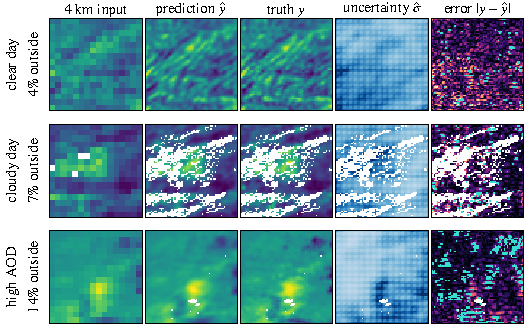
\includegraphics[width=\columnwidth]{final_paper/fig_examples_swinir.pdf}
\caption{SwinIR-light on three 2023 test patches (clear day, cloudy day, high AOD). From left: 4\,km input, 1\,km prediction \(\hat y\), true 1\,km map (these three share one color scale per row), predicted uncertainty \(\hat\sigma\) (model output, no truth used; darker = less sure), and actual error \(|y-\hat y|\). Cyan pixels fall outside the calibrated range \(\hat y\pm\hat\lambda\hat\sigma\); the row labels give their share. White pixels are clouds.}
\label{fig:examples}
\end{figure}

\subsection{RQ3: Is the Uncertainty Real, and Can It Be Trusted?}
A range of the same width everywhere can reach 90\% coverage without knowing which pixels are hard, so coverage alone cannot show that \(\hat\sigma\) is real uncertainty. Following recent work on SR uncertainty for satellite images~\cite{zheng2026selfsup} and on calibrated image-to-image uncertainty~\cite{angelopoulos2022im2im,belhasin2024puq}, we therefore answer RQ3 in two parts: (a) does \(\hat\sigma\) point at the pixels where the model is actually wrong, and (b) can it be turned into a range that is guaranteed to contain the true value for at least 90\% of pixels in an unseen year?

\textbf{(a) Does \(\hat\sigma\) track the error?} The NLL loss makes \(\hat\sigma^2\) an estimate of the expected squared error at each pixel~\cite{zheng2026selfsup}, and \(\hat\sigma\) is produced before the truth is seen. On 2023, pixels grouped by \(\hat\sigma\) show a 5--7\(\times\) rise in real RMS error from the most to the least confident group (Fig.~\ref{fig:rq3a}b). Across the 16 positions inside each \(4\times4\) block, the rank correlation between mean \(\hat\sigma\) and mean error is 0.99: block corners are harder than centers, and \(\hat\sigma\) learned this on its own. Per pixel, the rank correlation is 0.41--0.47. The size of \(\hat\sigma\), however, was only right for EDSR (90\% coverage 0.91). U-Net and SwinIR-light were overconfident (0.83 and 0.79; Fig.~\ref{fig:rq3a}a).

\begin{figure}[!t]
\centering
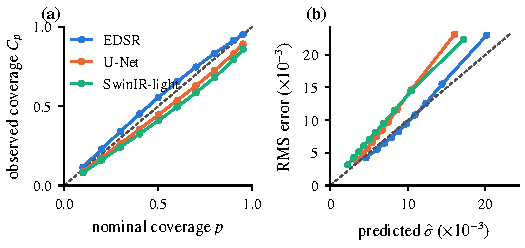
\includegraphics[width=\columnwidth]{final_paper/fig_rq3a_calibration.pdf}
\caption{RQ3(a) on 2023 (one run per model, epoch picked by RMSE). (a) Calibration curves; below the diagonal means overconfident. (b) Pixels grouped into ten equal bins by predicted \(\hat\sigma\), against their real RMS error; the error rises with \(\hat\sigma\) for every model, and the dashed line marks a perfectly sized \(\hat\sigma\).}
\label{fig:rq3a}
\end{figure}

\textbf{(b) A guaranteed 90\% range.} We form \(\hat y\pm\lambda\hat\sigma\) and choose \(\lambda\) on 2022 by conformal risk control~\cite{angelopoulos2022im2im,belhasin2024puq}. For each validation patch \(j\), let \(r_j(\lambda)\) be the fraction of its valid pixels outside the range. We take the smallest \(\hat\lambda\) with
\begin{equation}
\frac{1}{n}\sum_{j=1}^{n} r_j(\lambda) + \sqrt{\frac{\ln(1/\delta)}{2n}} \le \alpha ,
\end{equation}
with \(\alpha=\delta=0.1\) and \(n=1{,}142\). By Hoeffding's inequality, the expected miss rate on new data from the same distribution is then at most 10\% with 90\% confidence. (This \(\lambda\) is unrelated to the penalty weight in Section~III.) On 2023, every model misses only 6.5--7.2\% of pixels, so the guarantee holds. As a control, we calibrate a constant-width range \(\hat y\pm c\) the same way. Its average width is similar, but its misses concentrate on hard pixels: 17--20\% at cloud edges and on the 10\% highest-AOD patches, against 8--13\% for the \(\hat\sigma\)-based range (Fig.~\ref{fig:rq3b}). The \(\hat\sigma\) range is narrow where the model is reliable and wide where it is not, which is the evidence that \(\hat\sigma\) carries real per-pixel information.

\begin{figure}[!t]
\centering
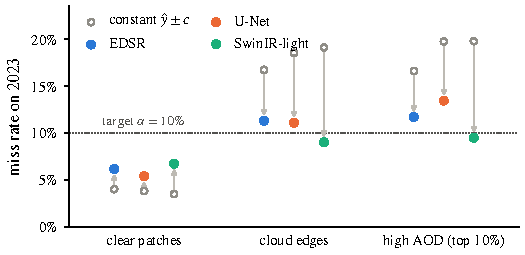
\includegraphics[width=\columnwidth]{final_paper/fig_rq3b_range.pdf}
\caption{RQ3(b) on 2023: miss rate by pixel group for each model, with both ranges calibrated on 2022 to the same guarantee (\(\le\)10\% misses with 90\% confidence). Arrows go from the constant range \(\hat y\pm c\) (open circles) to the \(\hat\sigma\)-based range \(\hat y\pm\hat\lambda\hat\sigma\) (filled). Using \(\hat\sigma\) cuts misses at cloud edges and on high-AOD patches from 17--20\% to 9--13\%, at a small cost on easy, clear patches.}
\label{fig:rq3b}
\end{figure}

\textbf{Why the original models were overconfident, and the fix.} Validation logs show that 2022 RMSE stops improving around epoch 30--75, but the network keeps shrinking \(\hat\sigma\) to fit the training years more closely: U-Net coverage on 2022 falls from 0.90 to 0.56 by epoch 200. Selecting the checkpoint by RMSE alone therefore picks an epoch where \(\hat\sigma\) is already too small. We compared four remedies, keeping the original runs (B0) as the baseline: M1 selects the epoch by 2022 NLL instead of RMSE and clips gradients at 1.0; M2 adds \(\beta\)-NLL with \(\beta=0.5\)~\cite{seitzer2022pitfalls}; M3 adds weight decay; and M4 is a deep ensemble of five M1 seeds~\cite{lakshminarayanan2017ensembles}, whose variance is the mean of the five \(\hat\sigma^2\) plus the spread of the five predictions. M2 and M3 were within seed-to-seed noise of M1 (single-seed coverage varies by up to 0.05), so Table~\ref{tab:methods} lists B0, M1, and M4.

\begin{table}[htbp]
\caption{RQ3 remedies on 2023. Cov.: raw 90\% coverage (target 0.90); \(\rho\): rank correlation of \(\hat\sigma\) and \(|y-\hat y|\); width and misses use the calibrated range \(\hat y\pm\hat\lambda\hat\sigma\) (honest \(\hat\lambda=1.645\)).}
\label{tab:methods}
\centering\footnotesize
\setlength{\tabcolsep}{2.5pt}
\resizebox{\columnwidth}{!}{%
\begin{tabular}{llccccccc}
\toprule
Model & & RMSE & Cov. & Cal.\,err. & \(\rho\) & \(\hat\lambda\) & Width & Miss \\
\midrule
U-Net & B0 & 0.0110 & 0.830 & 0.052 & 0.44 & 2.28 & 0.0333 & 7.0\% \\
 & M1 & 0.0111 & 0.850 & 0.033 & 0.45 & 2.20 & 0.0340 & 6.6\% \\
 & M4 & \textbf{0.0106} & 0.917 & 0.037 & \textbf{0.47} & \textbf{1.78} & \textbf{0.0321} & 6.4\% \\
\midrule
EDSR & B0 & 0.0116 & 0.912 & 0.033 & 0.41 & 1.75 & 0.0357 & 7.2\% \\
 & M1 & 0.0110 & 0.843 & 0.039 & 0.45 & 2.15 & 0.0332 & 7.4\% \\
 & M4 & \textbf{0.0106} & 0.892 & \textbf{0.014} & \textbf{0.46} & 1.88 & \textbf{0.0316} & 7.2\% \\
\midrule
SwinIR & B0 & 0.0107 & 0.791 & 0.083 & 0.47 & 2.53 & 0.0338 & 6.8\% \\
-light & M1 & 0.0107 & 0.872 & \textbf{0.014} & 0.46 & 2.02 & 0.0330 & 6.9\% \\
 & M4 & \textbf{0.0104} & 0.910 & 0.026 & \textbf{0.48} & \textbf{1.76} & \textbf{0.0303} & 7.2\% \\
\bottomrule
\end{tabular}}
\end{table}

Selecting the epoch by NLL (M1) removes most of the overconfidence at no extra cost for U-Net and SwinIR-light (SwinIR coverage 0.79\(\to\)0.87, calibration error 0.083\(\to\)0.014) and prevents a divergence that EDSR showed after epoch 110. For EDSR it trades a little coverage (0.91\(\to\)0.84) for better accuracy. The ensemble (M4) is the best overall: it has the lowest RMSE, the highest \(\rho\), coverage of 0.89--0.92, the smallest \(\hat\lambda\), and the narrowest calibrated range for every model. SwinIR-light M4 is the best single result (RMSE 0.0104, coverage 0.910, width 0.0303), at five times the training cost. Every method still meets the 90\% guarantee after calibration (6.4--7.7\% misses), and none reduces the misses at cloud edges (about 11\% for all), so the calibration step remains necessary.

% RQ4 on the year split: to be added (Rency).

\section{Discussion and Limitations}
Deep SR reliably sharpens 4\,km AOD toward the 1\,km MAIAC map, and the average-back constraint guarantees consistency with the coarse input without smoothing. The predicted uncertainty ranks hard pixels correctly but its raw size depends on training choices, so a calibration step on a held-out year is needed before it can be trusted. Several limits apply. A single network's \(\hat\sigma\) captures only data noise and misses ``never seen this'' uncertainty; the ensemble adds that and performs best. The guarantee assumes that 2023 behaves like 2022, and patches from the same day are correlated, so it is approximate. The ``truth'' is the 1\,km MAIAC product, so \(\hat\sigma\) measures distance from MAIAC, not from true aerosol or surface PM$_{2.5}$. Finally, the 4\,km inputs are created by averaging, and real coarse satellite products may behave differently~\cite{aybar2026sen2sr}. The RQ2 comparison and the B0 runs use one seed each; SwinIR seeds 1--4 were validated every 10 epochs rather than every 5.

\section{Conclusion}
On a strict year split, all three architectures beat bicubic by 8--15\% in RMSE, with SwinIR-light best across five seeds. The average-back constraint makes the output exactly consistent with the input at no cost in accuracy or detail. The predicted uncertainty points at the pixels the model gets wrong, and after one scale factor is calibrated on 2022, the resulting range contains the true value for over 90\% of 2023 pixels while placing its width where it is needed. Selecting the checkpoint by NLL removes most of the overconfidence for free, and a five-model ensemble gives the most accurate maps with honest to slightly cautious uncertainty.

% References start on their own, last page (\clearpage also places any remaining figures/tables first)
\clearpage
\bibliographystyle{IEEEtran}
\bibliography{refs}
\end{document}